\documentclass[aspectratio=169,10pt]{beamer}
\usetheme{default}
\usecolortheme{dove}
\setbeamertemplate{navigation symbols}{}
\setbeamertemplate{footline}[frame number]
\usepackage{booktabs}
\usepackage{graphicx}
\usepackage{xcolor}
\definecolor{scr}{HTML}{2a78d6}
\definecolor{rawc}{HTML}{eb6834}
\definecolor{refc}{HTML}{1baf7a}
\newcommand{\pass}{\textbf{pass}}
\newcommand{\fail}{\textbf{fail}}
\setbeamerfont{frametitle}{size=\large}

\title{Screening OPERA for hourly extremes}
\subtitle{Rules, how much each removes, what the reference data say}
\author{Filippo Quarenghi}
\date{14 October 2026}

\begin{document}

\begin{frame}
  \titlepage
\end{frame}

% ---------------------------------------------------------------------------------------------
\begin{frame}{The setting}
  \begin{itemize}
    \item \textbf{Target:} the 1-h accumulation at 2 km, OPERA's own ACRR convention:
      hour $H$ = $\tfrac14\times$(frames $H{-}45$, $H{-}30$, $H{-}15$, $H$).
    \item \textbf{Screening runs on the 15-min frames}: decide over the day, repair per frame,
      then sum. Tile-hours with clear errors are rejected when the splits are made.
    \item \textbf{Main concern:} unphysical values contaminating the extremes. Exact agreement of
      rain amounts with other products is secondary.
    \item \textbf{Ground rules}
      \begin{itemize}
        \item a rule is kept only if independent data support it (RADKLIM, DE/CH gauges);
        \item every pass criterion is written down and committed \emph{before} the test runs;
        \item no decision rests on looking at images.
      \end{itemize}
    \item \textbf{Data used here:} 199 calibration days (100 random, 79 event, 20 known
      failures); RADKLIM on 193 of them; gauges on 246 days.
  \end{itemize}
\end{frame}

% ---------------------------------------------------------------------------------------------
\begin{frame}{The rule set (current chain)}
  \footnotesize
  \begin{tabular}{lll}
    \toprule
    step & rule & how it is supported \\
    \midrule
    frame & drizzle $<0.1$ mm/h $\to 0$ & noise floor \\
    frame & static clutter (hot pixels, repair) & RADKLIM: 100\% of removals dry (89 cases) \\
    frame & spikes & signature \\
    frame & ceiling values (repair; $\ge 5$ px rejects the tile-hour) & context: 86\% not inside intense rain \\
    frame & footprints of $>500$ mm/h cores & physical bound \\
    frame & range rings $\ge 89$ mm/h & climatological geometry \\
    frames & RLAN rays (site-anchored, fixed over $\pm 4$ frames) & signature \\
    day & local-peak persistence ($p_1 \ge 24$ of 96 frames) & lowering it fails RADKLIM \\
    frame & cells without temporal support & RADKLIM: 97--100\% dry \\
    hour & isolated single-frame bursts & RADKLIM: 87.7\% dry \\
    split & radar-frame failures, repeated values, refused repairs & signature \\
    split & radar-day exclusion (score $\ge 1$) & RADKLIM: 99.8\% dry; rest of day worse \\
    \bottomrule
  \end{tabular}
\end{frame}

% ---------------------------------------------------------------------------------------------
\begin{frame}{How much each rule removes: random days (100)}
  \footnotesize
  Share of pixel-hours, by \emph{raw} hourly total, that the rule lowers by $\ge 50\%$.
  Rows ``rejected'' = pixel-hours dropped because their tile-hour is rejected.\\[4pt]
  \begin{tabular}{lrrrrr}
    \toprule
    rule & 5--10 mm & 10--20 & 20--50 & 50--100 & $\ge 100$ mm \\
    \midrule
    static clutter & 1.15\% & 4.31\% & \textbf{13.0\%} & \textbf{25.8\%} & \textbf{36.5\%} \\
    spikes & 0.60 & 1.22 & 2.17 & 3.51 & 6.57 \\
    ceiling repair & -- & -- & -- & 14.5 & 4.48 \\
    $>500$ mm/h footprints & -- & -- & 1.04 & 6.09 & \textbf{44.3} \\
    range rings & -- & -- & 0.11 & 8.76 & 1.89 \\
    persistence & 1.88 & 2.69 & 2.43 & 2.03 & 0.69 \\
    no temporal support & 0.22 & 0.38 & 0.91 & 0.94 & 0.18 \\
    bursts & -- & -- & 5.59 & 4.62 & 0.52 \\
    rejected: ceiling tile & 0.02 & 0.09 & 0.91 & 3.29 & 0.18 \\
    rejected: radar-day & 1.11 & 1.48 & 1.42 & 0.99 & 0.14 \\
    \midrule
    \textbf{left intact} & 95.0\% & 89.6\% & 71.9\% & 29.0\% & 4.2\% \\
    \bottomrule
  \end{tabular}\\[4pt]
  Below 5 mm: 98.5\% left intact. Hourly totals $\ge 100$ mm are rare in reality, so a 4\%
  survival there is expected.
\end{frame}

% ---------------------------------------------------------------------------------------------
\begin{frame}{How much each rule removes: event days (79)}
  \footnotesize
  Same measure on the days of the catalogued storms.\\[4pt]
  \begin{tabular}{lrrrrr}
    \toprule
    rule & 5--10 mm & 10--20 & 20--50 & 50--100 & $\ge 100$ mm \\
    \midrule
    static clutter & 0.63\% & 2.21\% & 8.25\% & \textbf{21.5\%} & 35.5\% \\
    spikes & 0.31 & 0.61 & 1.32 & 3.07 & 3.26 \\
    ceiling repair & -- & -- & -- & 7.03 & 6.02 \\
    $>500$ mm/h footprints & -- & -- & 0.47 & 6.00 & 24.0 \\
    range rings & -- & -- & 0.07 & 8.62 & 2.50 \\
    persistence & 0.91 & 1.49 & 2.62 & 4.32 & 1.41 \\
    no temporal support & 0.16 & 0.23 & 1.38 & \textbf{6.09} & 0.41 \\
    bursts & -- & -- & 2.67 & 4.72 & 0.68 \\
    rejected: unphysical & 0.01 & 0.08 & 0.87 & 0.74 & 19.0 \\
    rejected: ceiling tile & 0.02 & 0.07 & 0.67 & 6.43 & 0.66 \\
    rejected: radar-day & 0.89 & 1.22 & 1.54 & 1.25 & 0.17 \\
    \midrule
    \textbf{left intact} & 97.1\% & 94.0\% & 79.7\% & 30.3\% & 6.3\% \\
    \bottomrule
  \end{tabular}\\[4pt]
  Event days contain artefacts too: these are not real-rain losses as such. The tests on the next
  slide decide which are.
\end{frame}

% ---------------------------------------------------------------------------------------------
\begin{frame}{Is what each rule removes really an artefact?}
  \footnotesize
  RADKLIM presence test: a removal is ``dry'' when RADKLIM has $<5$ mm within $\pm 2$ px and
  $\pm 1$ h. Bar: $\ge 85\%$ dry. The disagreement floor of ordinary values is 5--6\%.\\[4pt]
  \begin{tabular}{llll}
    \toprule
    test & evidence & result & decision \\
    \midrule
    static-clutter repair & 89 removals, 100\% dry & \pass & stays \\
    no temporal support & 277 removals, 97--100\% dry & \pass & stays \\
    burst rule & 308 removals at 20--50 mm, 87.7\% dry & \pass & adopted \\
    isolated $\ge 31$ mm/h pixels (radar-day) & 69{,}726 pixel-frames, 99.8\% dry & \pass & stays \\
    rest of an excluded radar-day & false alarms 40\% vs 12\% (control) & worse & exclude whole day \\
    ceiling pixels & 13.7\% inside intense rain & artefacts & stays \\
    persistence $p_1$ 24 $\to$ 20 or 16 & 66--80\% dry, 24--59 confirmed real & \fail & stays 24 \\
    Mahalanobis outlier mask & 84\% / 76\% dry & \fail & not adopted \\
    radar-year exclusion & removed most event data & -- & dropped \\
    \bottomrule
  \end{tabular}\\[4pt]
  RADKLIM is reprocessed from the same German radars, so it can confirm an artefact both share.
  The tests cover Germany only; elsewhere rules rest on their signature.
\end{frame}

% ---------------------------------------------------------------------------------------------
\begin{frame}{Readiness gate before the full-archive build}
  \footnotesize
  \begin{tabular}{p{5.6cm}p{5.4cm}l}
    \toprule
    criterion & result & status \\
    \midrule
    1. known failures (Madrid, Valjevo, 48.62) kept & 0 / 0 / 0 tile-hours & \pass \\
    2a. false alarms vs RADKLIM at 20 mm, same gauge-hours & OPERA 6.3\%, RADKLIM 0.9\%: $+5.4$ points [$+2.3$, $+9.9$]; bar $\le +2$ & \fail \\
    2b. heavy gauge-hours the screen removes & 0.1\% & \pass \\
    3a. event tile-hours rejected & 0\% except on excluded radar-days & \pass \\
    3b. rejection rising with intensity & ceiling, radar-day: artefact-driven & explained \\
    3 / 5. tail stability, $\xi(u)$ drift & need the built test split & after build \\
    \bottomrule
  \end{tabular}\\[8pt]
  \textbf{The gate turns on 2a.} Of the 24 screened false-alarm gauge-hours, about 9 are clear
  artefacts (RADKLIM $\approx 0$). The largest: a stationary echo at Kleiner Feldberg on
  2018-04-30, 6 hours of 23--83 mm in a dry ring, a local peak in 20 frames (the threshold is 24).
  About 15 sit inside convection (RADKLIM 5--20 mm): most likely the gauge missed a small cell.
\end{frame}

% ---------------------------------------------------------------------------------------------
\begin{frame}{Distributions against gauges (point reference)}
  \centering
  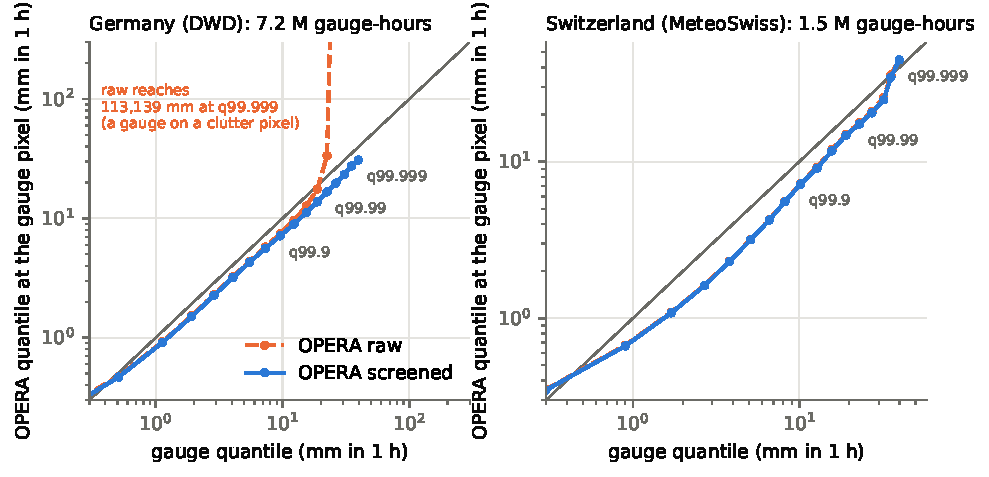
\includegraphics[width=0.92\textwidth]{figs/qq_gauges.pdf}\\
  \footnotesize\raggedright
  Quantiles of OPERA at the gauge pixel against the gauge, same gauge-hours (246 days).
  \textcolor{rawc}{Raw} OPERA in Germany is dominated above q99.99 by a gauge on a clutter pixel;
  \textcolor{scr}{screened} OPERA sits at 0.71--0.78$\times$ the gauge quantile from q99.9 to
  q99.999 (Switzerland 1.12$\times$ at q99.999, few cases): about 25\% low, from point vs 2 km area
  and radar underestimation.
\end{frame}

\begin{frame}{Exceedance against gauges}
  \centering
  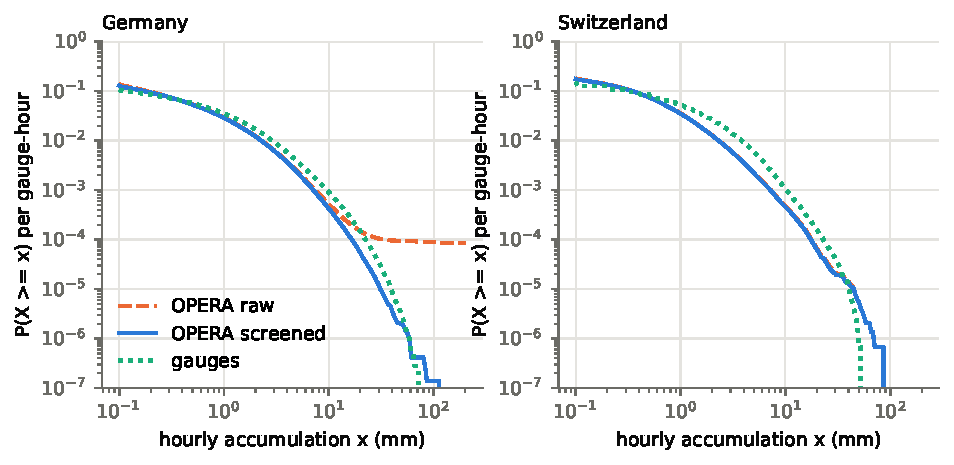
\includegraphics[width=0.92\textwidth]{figs/exceed_gauges.pdf}\\
  \footnotesize\raggedright
  $P(X \ge x)$ per gauge-hour. In Germany the screen removes a plateau of spurious values at
  $\sim 10^{-4}$; afterwards OPERA sits slightly below the \textcolor{refc}{gauges} at every level.
\end{frame}

\begin{frame}{Against RADKLIM on the same German pixel-hours}
  \centering
  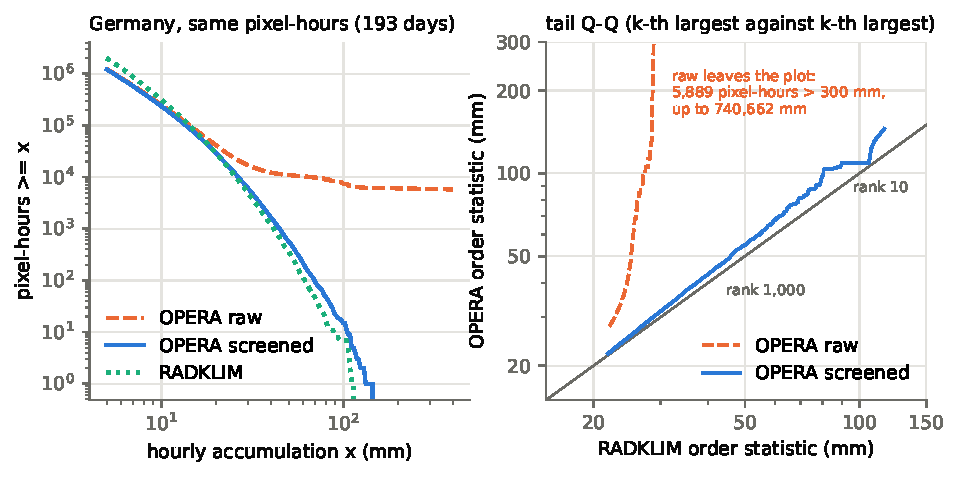
\includegraphics[width=0.92\textwidth]{figs/radklim.pdf}\\
  \footnotesize\raggedright
  Screened OPERA matches RADKLIM at 20 mm and has 1.2$\times$ / 1.6$\times$ / 2.5$\times$ its
  counts at 30 / 50 / 75 mm. RADKLIM underestimates peaks, so this excess bounds the residual
  contamination from above; it does not measure it.
\end{frame}

\begin{frame}{Europe: raw against screened (100 random days, full grid)}
  \centering
  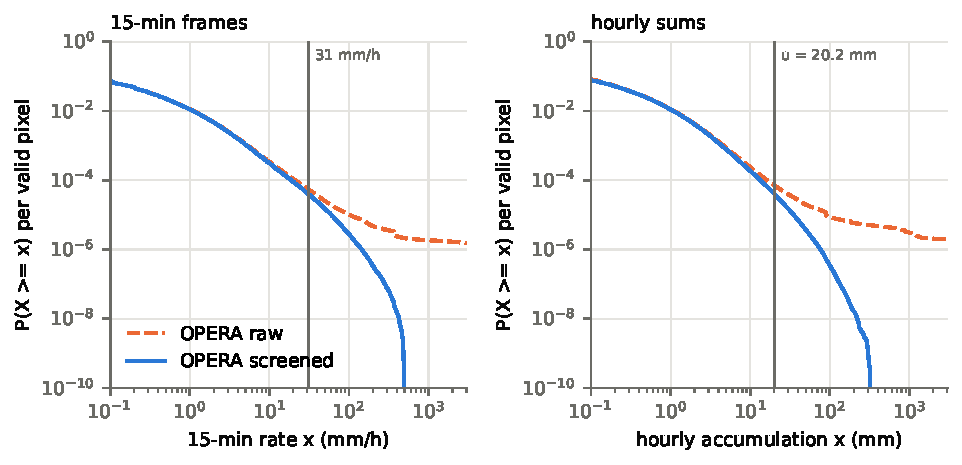
\includegraphics[width=0.92\textwidth]{figs/europe.pdf}\\
  \footnotesize\raggedright
  $P(X \ge x)$ per valid pixel. The screen leaves everything below $\sim 10$ mm/h (or mm) untouched
and cuts the spurious plateau of the \textcolor{rawc}{raw} tail, $10^{-6}$ to $10^{-5}$ up to
$10^3$; the \textcolor{scr}{screened} 15-min tail ends at the 500 mm/h physical bound.
\textbf{Provisional hourly tail threshold:} 31 mm/h is exceeded by $4.0\times10^{-5}$ of screened
15-min pixel-frames; the hourly sums exceed \textbf{$u$ = 20.2 mm} at the same frequency
(final $u$ from a stability analysis on the build).

\end{frame}

% ---------------------------------------------------------------------------------------------
\begin{frame}{Decisions this week}
  \small
  \begin{itemize}
    \item Radar ownership from the radars listed in each composite (Italy never contributes;
      Austria never; CH and HU from 2014).
    \item Radar-day exclusion by a pre-stated score ($\ge 1$, one decade above both the radar's
      own seasonal q99 and its neighbours); \textbf{radar-year rule dropped}.
    \item Static-clutter repair and the temporal-support rule \textbf{kept}; persistence
      threshold \textbf{kept at 24}.
    \item \texttt{min\_wet\_jump} 0.15 $\to$ 0.021, now derived (q99.9 of normal operation);
      same 48 flagged frames.
    \item Burst rule adopted; Mahalanobis mask not adopted.
  \end{itemize}
\end{frame}

\begin{frame}{Limitations to state}
  \small
  \begin{itemize}
    \item Independent data cover Germany and Switzerland only; elsewhere rules rest on their
      signature (Valjevo, Madrid and Oradea lie outside).
    \item RADKLIM shares the German radars and checks presence, not magnitude.
    \item The screen targets overestimation: blockage, attenuation and overshoot (Alps) are not
      corrected, so the tail is biased low there.
    \item Up to about a third of kept values $\ge 75$ mm over Germany are RADKLIM-dry.
    \item The plain hourly sum beads fast cells; the advection-corrected field is stored alongside.
    \item Criteria were fixed in advance internally (commit timestamps), not registered externally.
  \end{itemize}
\end{frame}

\begin{frame}{Next steps}
  \small
  \begin{enumerate}
    \item A rule for single-day stationary echoes (fixed location, dry ring, many hours): the
      remaining cause of the 2a failure. Test it like the others.
    \item Full-archive hourly scan ($\sim 30$ h), splits and store.
    \item Gate criteria 3 and 5 on the build; hourly tail threshold from a stability analysis.
    \item Retrain the backbones on v4 and recompute $\sigma_r$.
  \end{enumerate}
\end{frame}

\end{document}
